\documentclass[9pt]{beamer}
\mode<presentation>

% Theme choice:
\usetheme{Madrid}%Darmstadt 

\usecolortheme[RGB={0,100,50}]{structure}
 
\setbeamercovered{invisible}
%\setbeamertemplate{navigation symbols}{}
\usepackage{dynblocks}
\usepackage{textpos}
\usepackage{pifont}
\usepackage{amsfonts}
\usepackage{amsmath}
\usepackage{amssymb}
\usepackage{amsthm}
\usepackage{mathtools}
\usepackage{hyperref}
\usepackage[utf8]{inputenc}
\usepackage[T1]{fontenc}
\usepackage[usestackEOL]{stackengine}
\usepackage{mdframed}

\usepackage[affil-it]{authblk} 
\usepackage{etoolbox}
\usepackage{lmodern}
\usepackage{listings}
\usepackage{tikz}
\usetikzlibrary{positioning}
\usetikzlibrary{shapes.geometric}
\usetikzlibrary{calc}

\usepackage{caption}
\usepackage{subcaption}

\usepackage{xcolor}
\usepackage[usestackEOL]{stackengine}
\usepackage{lipsum}
\usepackage{pifont}

\usefonttheme{serif} 
\newmdtheoremenv{theo}{Theorem}
\newcommand{\xmark}{\ding{55}}

\makeatletter
\patchcmd{\@maketitle}{\LARGE \@title}{\fontsize{18}{19.2}\selectfont\@title}{}{}
\makeatother

\renewcommand\Authfont{\fontsize{12}{14.4}\selectfont}
\renewcommand\Affilfont{\fontsize{9}{10.8}\itshape}

% Title page details: 
\title[Presentation]{Dearrangement} %add title


\institute[BUET]{\textbf{
    \large Md. Ashrafur Rahman Khan | 1905005
    \\Md. Nabil Sadique  | 1905006
    \\Md. Asib Rahman | 1905007
    \hspace{0.5pt}
    \\ \qquad
    \\ \hspace{1pt}
    \\
\includegraphics[width=1cm]{buet_logo.png}
    \\\hspace{.3pt}
    \\ CSE300 Presentation
    \\ \hspace{.3pt}
    \\Department of CSE | BUET}
} 
\date{\today}

\usepackage[pscoord]{eso-pic}

\newcommand{\drawBooks}[4]{
\begin{tikzpicture}
    \foreach \x/\y/\z/\w in {0/#1/A, 3/#2/B, 6/#3/C, 9/#4/D}
        {
            \node at (\x+.8, 2.4) {\w}; 
            \fill[color=\y] (\x,0) rectangle +(1.5,2);
            \draw (\x,0) rectangle +(1.5,2);
            \draw (\x,0) .. controls (\x, -.147) and (\x+.082, -.238)  .. (\x+.15, -.25) -- ++(1.53, 0) -- ++(0, 2) -- 
            (\x+1.5,2);
            \node at (\x+.7, 1.5) {\small\z's book};
            % \draw (\x+1.5, 0) -- (\x+1.68, -.25); 
        }
\end{tikzpicture}
}

\newcommand{\drawCenteredBooks}[4]{
    \begin{figure}
        \centering
        \drawBooks{#1}{#2}{#3}{#4}
    \end{figure}
}

\newcommand{\drawThreeDeramgent}{
\begin{figure}
    \centering
    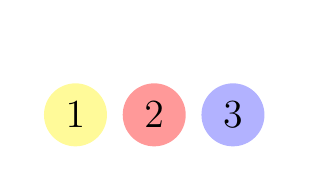
\begin{tikzpicture}
        \draw[white] (0,0) grid (3,1);
        \draw[white] (-.1,-.1) rectangle (3.1,1.1);
        \foreach \i/\j in {1/yellow!40, 2/red!40, 3/blue!30}
        {
            \fill[\j] (\i-.5, 0) circle (.4); 
            \node at (\i-.5, 0) {\Large \i};
        }
    \end{tikzpicture}
    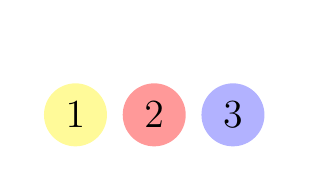
\begin{tikzpicture}
        \draw[white] (0,0) grid (3,1);
        \draw[white] (-.1,-.1) rectangle (3.1,1.1);
        \foreach \i/\j in {1/yellow!40, 2/red!40, 3/blue!30}
        {
            \fill[\j] (\i-.5, 0) circle (.4); 
            \node at (\i-.5, 0) {\Large \i};
        }
    \end{tikzpicture} \\
    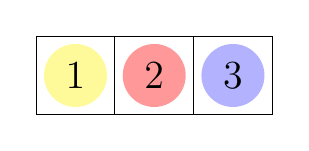
\begin{tikzpicture}
        \draw (0,0) grid (3,1);
        \draw[white] (-.1,-.1) rectangle (3.1,1.1);
        \foreach \i/\j/\k in {1/1/yellow!40, 2/2/red!40, 3/3/blue!30}
        {
            \fill[\k] (\i-.5, .5) circle (.4);
            \node at (\i-.5, .5) {\Large \j};
        }
    \end{tikzpicture} 
    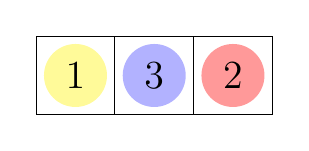
\begin{tikzpicture}
        \draw (0,0) grid (3,1);
        \draw[white] (-.1,-.1) rectangle (3.1,1.1);
        \foreach \i/\j/\k in {1/1/yellow!40, 2/3/blue!30, 3/2/red!40}
        {
            \fill[\k] (\i-.5, .5) circle (.4);
            \node at (\i-.5, .5) {\Large \j};
        }
    \end{tikzpicture} \\
    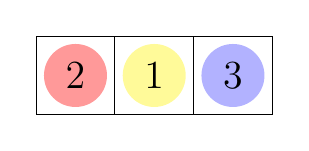
\begin{tikzpicture}
        \draw (0,0) grid (3,1);
        \draw[white] (-.1,-.1) rectangle (3.1,1.1);
        \foreach \i/\j/\k in {1/2/red!40, 2/1/yellow!40, 3/3/blue!30}
        {
            \fill[\k] (\i-.5, .5) circle (.4);
            \node at (\i-.5, .5) {\Large \j};
        }
    \end{tikzpicture}  
    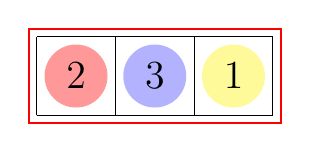
\begin{tikzpicture}
        \draw (0,0) grid (3,1);
        \uncover<5->{
            \draw[red, thick] (-.1,-.1) rectangle (3.1,1.1);
        }
        \foreach \i/\j/\k in {1/2/red!40, 2/3/blue!30, 3/1/yellow!40}
        {
            \fill[\k] (\i-.5, .5) circle (.4);
            \node at (\i-.5, .5) {\Large \j};
        }
    \end{tikzpicture} \\
    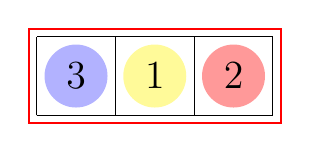
\begin{tikzpicture}
        \draw (0,0) grid (3,1);
        \uncover<5->{
            \draw[red, thick] (-.1,-.1) rectangle (3.1,1.1);
        }
        \foreach \i/\j/\k in {1/3/blue!30, 2/1/yellow!40, 3/2/red!40}
        {
            \fill[\k] (\i-.5, .5) circle (.4);
            \node at (\i-.5, .5) {\Large \j};
        }
    \end{tikzpicture} 
    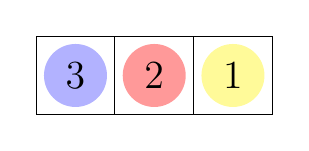
\begin{tikzpicture}
        \draw (0,0) grid (3,1);
        \draw[white] (-.1,-.1) rectangle (3.1,1.1);
        \foreach \i/\j/\k in {1/3/blue!30, 2/2/red!40, 3/1/yellow!40}
        {
            \fill[\k] (\i-.5, .5) circle (.4);
            \node at (\i-.5, .5) {\Large \j};
        }
    \end{tikzpicture}
    \caption{All Derangements}
\end{figure}
}

\begin{document}

% \setbeamercolor{background canvas}{bg=blue!20}

% Title page frame
\begin{frame}
    \titlepage 
\end{frame}

% %logo
% \AddToShipoutPictureFG{
%     \put(\LenToUnit{.92\paperwidth},
%     \LenToUnit{.185\paperheight})
%     {\vtop{{\null}
%     \makebox{
\includegraphics[width=.8cm,keepaspectratio]{buet_logo.png}}}}
%     }


\begin{frame}{Outline}
  \tableofcontents
\end{frame}

\section{Introduction}

\subsection{A problem}
\begin{frame}{A problem}
    \begin{example}
        There are 4 book-worm friends. They read books like maniac. Once in every month they meet each other and exchange their books. One of the friends who read a mathematics book recently thought what is the total number of ways they can exchange books?
    \end{example}
    

    \begin{columns}
        \column{.5\textwidth}<2->
        Constraints: \\ 
        No one should get the book s/he brought.

        \column{.4\textwidth}
        \begin{figure}
            \centering
            
\includegraphics[width=.7\textwidth]{book_exchange.jpeg}
            \label{fig:book_exchange}
            \caption{Two Friends exchanging books}
        \end{figure}
    \end{columns}
\end{frame}

\begin{frame}{Example Elaborated}
    \begin{example}
        Let, 4 friends A , B ,C and D had came to Book Exchange Party.
        They want to exchange them...
    \end{example}
    \qquad
    \vspace{2pt}
    \only<1>{
        \drawCenteredBooks{green!20/A}{red!20/B}{blue!20/C}{yellow!40/D} 
    }
    \only<2>{
        \drawCenteredBooks{red!20/B}{yellow!40/D}{blue!20/C}{green!20/A}
    }
    \only<3>{
        \drawCenteredBooks{blue!20/C}{red!20/B}{yellow!40/D}{green!20/A}
    }
    \only<4>{
        \drawCenteredBooks{blue!20/C}{yellow!40/D}{green!20/A}{red!20/B}
    }
    \only<5>{
        \drawCenteredBooks{yellow!40/D}{red!20/B}{green!20/A}{blue!20/C}
    }

    \qquad
    \centering{
        \only<4,5>{\large\textcolor{green}{\checkmark }Derangement}
        \only<1,2,3>{\large\textcolor{red}{\xmark } Not a Derangement}
    }
\end{frame}

\subsection{Definition}
\begin{frame}{What is Derangement}

\begin{Definition}[Dearangement]
    In combinatorial mathematics, a derangement is a permutation of the elements of a set, such that no element appears in its original position.
\end{Definition}

\begin{columns}
    \column{.4\textwidth}
        \begin{itemize}
            \item<2-> Dearrangement is a permutation with no elements in their natural place.
            \item<3-> Mathematically, the number of derangements of a set of $n$ elements is expressed as, $ !n $
            \item<5-> For example, \Large $!3 = 2$.
        \end{itemize}   
    \column{.6\textwidth}<4->
    \drawThreeDeramgent
      
\end{columns}

\end{frame}

\subsection{Examples}

\begin{frame}{More Examples}
    \vspace{1cm}
    \begin{columns}

        \column{.4\textwidth}
        To check exam scripts faster, a teacher uses his/her students to check scripts. At first s/he distributes the scripts to all students such that no student got their own scripts. How many ways s/he can do that?
        \vspace{0.5cm}
        \begin{figure}
            \centering
            
\includegraphics[width=0.5\textwidth]{exam_02.jpeg}
            \label{fig:exam_scripts}
        \end{figure}

        \pause

        \column{.4\textwidth}
        You were putting named invitation cards to envelope for your birthday. Suddenly a problem popped to your mind that if envelops are filled randomly what is the probability that no envelop will be in the right place?
        \vspace{0.5cm}
        \begin{figure}[b]
            \centering
            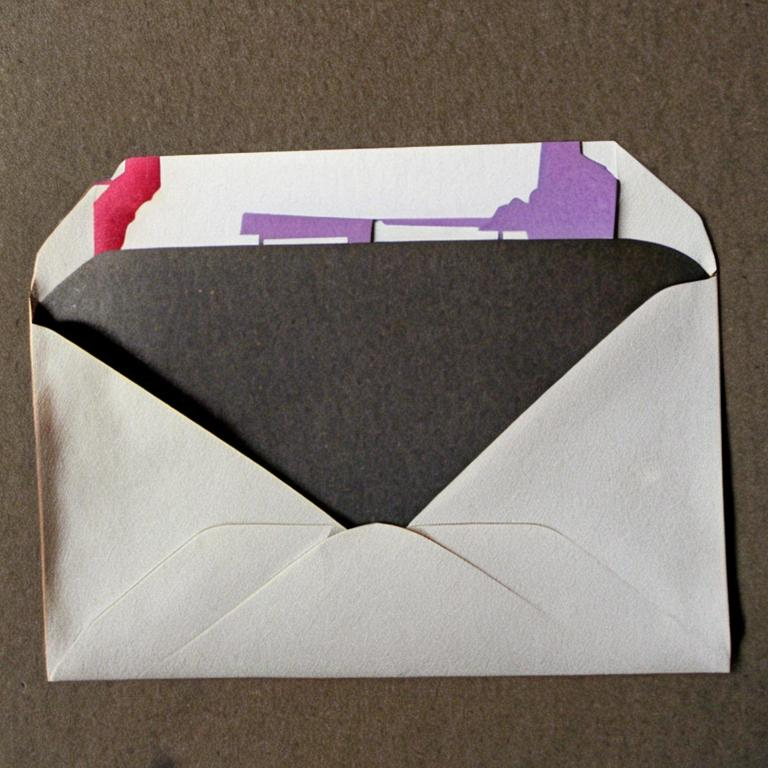
\includegraphics[width=0.5\textwidth]{envelope.jpeg}
            \label{fig:envelope}
        \end{figure}
    \end{columns}
    
\end{frame}


\section{Recursive Definition}
\subsection{Formulation}

\tikzstyle{box}=[rectangle, draw=black,
           text centered, text=black, minimum width=1cm, minimum height=1cm]
\tikzstyle{mbox}=[rectangle, draw=blue, thick, fill=blue!5,
           text centered, text=black, minimum width=2cm, minimum height=1.25cm]
\begin{frame}
\centering
\Huge \textbf{ How to find derangements? }
\end{frame}

\begin{frame} {Recursive Formulation}
    \Large {\textbf{Base case ($n = 1$)}} \\
    \vspace{1cm}
    \begin{figure}
        \centering
        \begin{tikzpicture}
            \node[box, fill=blue!20] at (0,0) {$ a_1 $};
            \pause
            \node[mbox] at (0, -2) {$ !1 = 0$};
        \end{tikzpicture}
    \end{figure}
\end{frame}


\begin{frame} {Recursive Formulation}
    \Large {\textbf{Base case ($n = 2$)}} \\
    \vspace{1cm}
    \begin{figure}
        \centering
        \begin{tikzpicture}
            \node[box, fill=blue!20] at (0,0) {$ a_1 $};
            \node[box, fill=red!20] at (1.25,0) {$ a_2 $};
            \pause
            \node[box, fill=red!20] at (0,-2.5) {$ a_2 $};
            \node[box, fill=blue!20] at (1.25,-2.5) {$ a_1 $};

            \draw[->, thick] (0.62, -0.75) --++ (0, -1);
            \pause
            \node[mbox] at (5, -1.35) {$!2 = 1$};
        \end{tikzpicture}
    \end{figure}
\end{frame}


\begin{frame} {Recursive Formulation}
    \begin{block}{Recursive Case}
        For $n \ge 2$
    \end{block}
    \vspace{1cm}
    \begin{figure}
        \centering
        \begin{tikzpicture}
            \draw[fill=blue!10] (0.5,-1) rectangle (8, 1);
            \foreach \x in {1, 2, 3, 4}
            {
                \node[box, fill=green!10](a_\x) at (\x + \x * 0.25,0) {$ a_\x $};

            }
            \node at (6, 0) {...};
            \node[box, fill=green!10] (a_n_1) at (7 ,0) {$ a_{n-1} $};
            \node[box, fill=red!10] (a_n) at (9,0) {$ a_{n} $};
            \pause
            \draw[ ->] (a_n) edge [bend left] (a_1.south);
            \draw[ ->] (a_n) edge [bend left] (a_2.south);
            \draw[ ->] (a_n) edge [bend left] (a_3.south);
            \draw[ ->] (a_n) edge [bend left] (a_4.south);
            \draw[ ->] (a_n) edge [bend left] (a_n_1);

        \end{tikzpicture}
    \end{figure}
\end{frame}

\begin{frame} {Recursive Formulation}
    \begin{block} {Case 1}
        $a_1$ at $n$th position, $a_n$ at 1st position
    \end{block}

    \begin{figure}
        \centering
        \begin{tikzpicture}
            \uncover<4-> {\draw[fill=blue!10] (1.85,-1) rectangle (7.7, 1);}
            \foreach \x in {2, 3, 4}
            {
                \node[box, fill=green!10](a_\x) at (\x + \x * 0.25,0) {$ a_\x $};

            }
            \node at (6, 0) {...};
            \node[box, fill=green!10] (a_n_1) at (7,0) {$ a_{n-1} $};
            \only<1>{
                \node[box, fill=red!10] at (9,0) {$ a_{n} $};
            }
            \only<2->{
                \node[box, fill=green!10] (a_n) at (9,0) {$ a_{1} $};
            }
            \uncover<2-3> {
                \draw[ ->] (a_n) edge [bend left] (a_1.south);
            }
            \uncover<3> {
                \draw[ ->] (a_1.north) edge [bend left] (a_n);
            }
            \only<1>{
                \node[box, fill=green!10] at (1.25,0) {$ a_1 $};
            }
            \only<2->{
                \node[box, fill=red!10] (a_1) at (1.25,0) {$ a_n $};
            }
            \uncover<5-> {
                \node at (4.75, -1.5) {$!(n-2)$};
            }
        \end{tikzpicture}
    \end{figure}
\end{frame}

\begin{frame} {Recursive Formulation}
    \begin{block} {Case 2}
        $a_1$ at $n$th position, $a_n$ at $i$th position ($i \neq 1 $)
    \end{block}

    \begin{figure}
        \centering
        \begin{tikzpicture}
            \uncover<3->{
                \draw[fill=blue!10] (0.5,-1) rectangle (8, 1);
            }
            \foreach \x in { 2, 3, 4}
            {
                \node[box, fill=green!10](a_\x) at (\x + \x * 0.25,0) {$ a_\x $};

            }
            \node at (6, 0) {...};
            \node[box, fill=green!10] (a_n_1) at (7,0) {$ a_{n-1} $};
            \node[box, fill=green!10] (a_n) at (9,0) {$ a_{1} $};
            \node[box, fill=red!10] (a_1) at (1.25,0) {$ a_n $};
            \uncover<2> {
                \draw[ ->] (a_1) edge [bend right] (a_2.south);
                \draw[ ->] (a_1) edge [bend right] (a_3.south);
                \draw[ ->] (a_1) edge [bend right] (a_4.south);
                \draw[ ->] (a_1) edge [bend right] (a_n_1.south);
            }
            \uncover<4-> {
                \node at (4, -1.5) {$!(n-1)$};
            }
        \end{tikzpicture}
    \end{figure}
\end{frame}

\begin{frame} {Recursive Formulation}
    \begin{block}{Recursive Formula}
        \begin{align*}
            !n = \uncover<2-> {
                    \uncover<4> {
                        (n - 1) (
                    }
                    !(n-2)
                    \uncover<3-> {
                       \quad + \quad !(n-1)
                    }
                \uncover<4-> {
                    )
                }
            }
        \end{align*}
    \end{block}
    \vspace{1cm}
    \uncover<3-4>{
        \begin{figure}
        \centering
        \begin{tikzpicture}
            \draw[fill=blue!10] (0.5,-1) rectangle (8, 1);
            \foreach \x in {1, 2, 3, 4}
            {
                \node[box, fill=green!10](a_\x) at (\x + \x * 0.25,0) {$ a_\x $};

            }
            \node at (6, 0) {...};
            \node[box, fill=green!10] (a_n_1) at (7 ,0) {$ a_{n-1} $};
            \node[box, fill=red!10] (a_n) at (9,0) {$ a_{n} $};
            \pause
            \draw[ ->] (a_n) edge [bend left] (a_1.south);
            \draw[ ->] (a_n) edge [bend left] (a_2.south);
            \draw[ ->] (a_n) edge [bend left] (a_3.south);
            \draw[ ->] (a_n) edge [bend left] (a_4.south);
            \draw[ ->] (a_n) edge [bend left] (a_n_1);

        \end{tikzpicture}
        \end{figure}
    }

\end{frame}

\subsection{Code}

\begin{frame}[fragile]{Recursive Function}
\begin{block}{C++ function}
\begin{lstlisting}[language=C++]
    int derangement(int n) {
        if(n == 1) return 0;
        if(n == 2) return 1;
        return (n - 1) * (derangement(n - 1)
                        + derangement(n - 2));
    }
\end{lstlisting}
\end{block}
\end{frame}

\section{Mathematical Formula}

\begin{frame}{Closed Form Formula}
    \centering
    \LARGE  \textbf{ A Closed Form Formula for Derangement }
\end{frame}


\begin{frame}{Inclusion-Exclusion}
    \begin{theo}[Inclusion-Exclusion theorem]
    In combinatorics, a branch of mathematics, the inclusion–exclusion principle is a counting technique which generalizes the familiar method of obtaining the number of elements in the union of two finite sets; symbolically expressed as
    \[|A\cup B| = |A|+|B|-|A \cap B|\]
    \end{theo}
    \centering
    \vspace{1cm}
    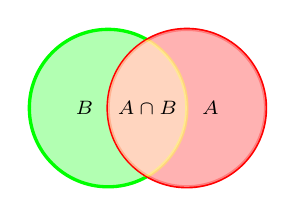
\begin{tikzpicture}
        \begin{scope}[blend group=soft light]
        \fill[red!30!white]  (0:0.5) circle (1);
        \draw[red , very thick] (0:0.5) circle (1);
        \draw[green , very thick] (180:0.5) circle (1);
        \fill[green!30!white] (180:0.5) circle (1);
        \end{scope}
        \node at (0:0.8) {\scriptsize{$A$}};
        \node at (180:0.8) {\scriptsize{$B$}};
        \node at (0:0) {\scriptsize{$A\cap B$}};
    \end{tikzpicture}
\end{frame}


\begin{frame}{Inclusion-Exclusion For Three Sets}

\begin{columns}
\column{0.5\textwidth}<2->
\begin{alertblock}{For Three sets A , B , C}
$|A\cup B\cup C|=|A|+|B|+|C|-\newline |A\cap B|-|A\cap C|-|B\cap C|+|A\cap B\cap C|$
\end{alertblock}
Here \textbf{$|A \cap B \cap C|$} = Number of elements in union of sets A , B , C

\column{0.5\textwidth}<1->
\begin{figure}
    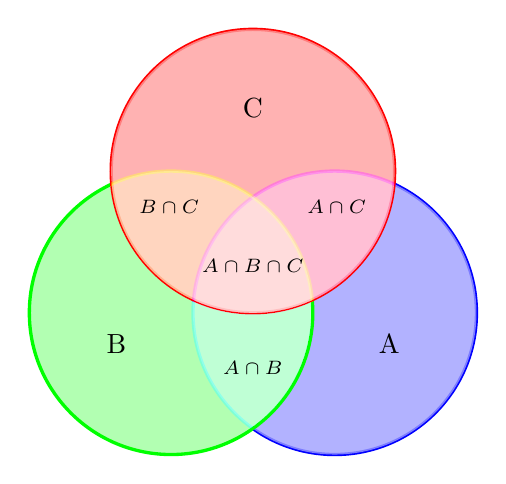
\begin{tikzpicture}
    \begin{scope}[blend group=soft light]
    \fill[red!30!white]  ( 90:1.2) circle (1.8);
    \draw[red , very thick] (90:1.2) circle (1.8);
    \draw[green , very thick] (210:1.2) circle (1.8);
    \fill[green!30!white] (210:1.2) circle (1.8);
    \fill[blue!30!white]  (330:1.2) circle (1.8);
    \draw[blue , very thick] (330:1.2) circle (1.8);
    \end{scope}
    \node at ( 90:2)    {C};
    \node at (210:2)    {B};
    \node at (330:2)    {A};

    \node at (35:1.3) {\scriptsize{$A\cap C$}};
    \node at (145:1.3) {\scriptsize{$B\cap C$}};
    \node at (270:1.3) {\scriptsize{$A\cap B$}};
    \node  {\scriptsize{$A\cap B\cap C$}};


\end{tikzpicture}

    \pause

    \caption{Venn Diagram for three sets}
    \label{fig:my_label}
\end{figure}


\end{columns}

\end{frame}

\begin{frame}{Some Necessary Information}
\begin{table}
    \centering
    \begin{tabular}{|c|c|}
    \hline
    \textbf{Symbol} & \textbf{Number of element matching}\\ \hline
    $\sum_i \left|S_i\right|$ &  $1$\\ \hline
    $\sum_{i < j} \left|S_i \cap S_j\right|$ & $2$\\ \hline
    $\vdots$ & $\vdots$ \\ \hline
    $\sum_{i < j < \cdots < k} \left|S_i \cap S_j \cap \cdots \cap S_k\right|$ & $k$ \\ \hline
     \end{tabular}
    \caption{Meaning of the symbol}
    \label{tab:my_label}
\end{table}


\end{frame}

\begin{frame}{Derivation of Formula}
    \begin{align*}
     \left|S_1 \cup \dotsm \cup S_n\right|
  &= \sum_i \left|S_i\right|
    - \sum_{i < j} \left|S_i \cap S_j\right|
    + \sum_{i < j < k} \left|S_i \cap S_j \cap S_k\right|
    + \\
  & \hspace{0.5cm} \cdots +(-1)^{n + 1} \left|S_1 \cap \dotsm \cap S_n\right|\\
  &= \binom{n}{1}(n - 1)! - \binom{n}{2}(n - 2)! + \binom{n}{3}(n - 3)! - \\
  &  \hspace{0.5cm} \cdots + (-1)^{n+1}\binom{n}{n} 0!\\
  &= \sum_{i=1}^n (-1)^{i+1}\binom{n}{i}(n - i)!\\
  &= n!\ \sum_{i=1}^n {(-1)^{i+1} \over i!},
\end{align*}

\end{frame}


\begin{frame}{Derivation of Formula}
And since a derangement is a permutation that leaves none of\\
the n objects fixed, this implies -\\
\vspace{1cm}
\centering
\begin{tikzpicture}
    \node[mbox, text width=8cm] at (0,0) {
        \[ !n=n!-\left|S_{1}\cup \dotsm \cup S_{n}\right|=n!\sum _{i=0}^{n}{\frac {(-1)^{i}}{i!}}.\]
    };
\end{tikzpicture}

\end{frame}

\begin{frame}{References}

\begin{itemize}

    \item[$\blacksquare$] Derangement - Wikipedia
    \item[$\blacksquare$] Inclusion-Exclusion Principle - Wikipedia
\end{itemize}

\end{frame}




\end{document}
